% Provenance (never printed): old premiere S material on subduction (Wadati-Benioff
% planes, density of the old lithosphere, slab pull, transformation of the slab at
% depth: blueschist and eclogite; anatomy of an active margin). Sections from
% figdata/grade-11/slab_sections.py (USGS ComCat M >= 6 1976-2025, PB2002 steps,
% Seton 2020 ages); plate speeds from plate_velocities.py (NNR-MORVEL56 RMS).
% Metamorphism is defined in g12.03, the volcanic arc in g12.04: named only here.
\chapter{As zonas de subducção}\label{ch:g11:subduction-zones}

Sob as ilhas de Tonga, no sudoeste do Pacífico, a Terra treme muito mais
fundo do que em qualquer outro lugar. Dos sete mil terremotos de magnitude 6
ou mais registrados no mundo entre 1976 e 2025, o mais profundo aconteceu a
\qty{688}{km} de profundidade, e o corte através de Tonga deste capítulo
contém eventos até cerca de \qty{671}{km}. A essas profundidades, a rocha é
quente e está sob uma pressão enorme; ela deveria escoar lentamente, como a
\omterm{def:g11:lithosphere-asthenosphere:lithosphere}{astenosfera}, e não se romper. No entanto, ela se rompe. Este capítulo
explica o que existe ali para se romper: uma \omterm{def:g11:subduction-zones:slab}{laje} de fundo oceânico frio que
afunda de volta no manto.
% ledger: data:usgs-comcat (catalogue_maxdepth 688; tonga_maxdepth 670.8, slab_sections.py)

\begin{recall}
Num limite convergente, duas placas se movem uma em direção à outra; fossas
profundas acompanham algumas delas (Livro 1, 7º e 8º anos). A magnitude de
um terremoto mede o seu tamanho, e um terremoto sob o mar pode provocar um
tsunami (Livro 1, 7º ano). A velocidade de uma placa em relação a outra é a
diferença das suas velocidades (\cref{ch:g11:plate-motions}). O fundo
oceânico afunda à medida que envelhece, e depois de uns 60 milhões de anos a
sua \omterm{def:g11:lithosphere-asthenosphere:lithosphere}{litosfera}, com cerca de \qty{100}{km} de espessura, é mais densa que a
\omterm{def:g11:lithosphere-asthenosphere:lithosphere}{astenosfera} abaixo dela (\cref{ch:g11:ocean-ridges}). As ondas sísmicas
mostram uma mudança brusca no manto a cerca de \qty{670}{km}
(\cref{ch:g11:seismic-structure}). Uma rocha metamórfica é uma rocha
transformada no estado sólido (Livro 1, 6º ano).
\end{recall}
% ledger: data:prem (670 km), ps77:depth-age

\section{Fossas e zonas inclinadas de terremotos}

A maioria dos terremotos é rasa: no catálogo dos de magnitude 6 ou mais desde
1976, apenas cerca de um em cinco tem mais de \qty{70}{km} de profundidade, e
um em quinze mais de \qty{300}{km}. O mapa abaixo mostra onde ficam os
profundos.
% values (slab_sections.py): frac_deeper_70 0.21, frac_deeper_300 0.069; data:usgs-comcat

\begin{omfigure}
\begin{tikzpicture}
\begin{axis}[ommap, width=\linewidth, xtick={-180,-90,...,180}, ytick={-60,0,60},
  legend style={font=\scriptsize, at={(0.5,-0.13)}, anchor=north, legend columns=3,
    /tikz/every even column/.append style={column sep=6pt}}]
\addplot[fill=omLithAlluv, draw=black!45, line width=0.2pt, forget plot] table {figdata/out/shared-geo-land.dat};
\addplot[black!70, line width=0.5pt, forget plot] table {figdata/out/shared-geo-school-subduction.dat};
\addplot[fill=black!70, draw=none, forget plot] table {figdata/out/shared-geo-school-teeth.dat};
% computed in figdata/grade-11/slab_sections.py; ledger: data:usgs-comcat, data:pb2002
\addplot[only marks, mark=*, mark size=0.55pt, black!45] table[x=lon, y=lat] {figdata/out/grade-11-slab_sections-world-shallow.dat};
\addplot[only marks, mark=*, mark size=0.8pt, omProp] table[x=lon, y=lat] {figdata/out/grade-11-slab_sections-world-mid.dat};
\addplot[only marks, mark=*, mark size=1.1pt, omThm] table[x=lon, y=lat] {figdata/out/grade-11-slab_sections-world-deep.dat};
\legend{{menos de \qty{70}{km}}, {de 70 a \qty{300}{km}}, {mais de \qty{300}{km}}}
\end{axis}
\end{tikzpicture}

{\small Terremotos de magnitude 6.5 ou mais, 1976--2025 (2192 eventos),
coloridos pela profundidade, com as fossas (linha preta, triângulos sobre a
placa que se sobrepõe). Os terremotos intermediários e profundos ficam
apenas ao longo de algumas fossas, sempre do lado da placa que se sobrepõe.
Dados: catálogo de terremotos do USGS; limites de placas de Bird (2003);
terras emersas de Natural Earth.}
\end{omfigure}
% values: world_n_m65 2192, world_deep_n 197 (slab_sections.py)

Os terremotos profundos não estão espalhados: eles seguem as fossas do
Pacífico ocidental, de Kamchatka ao Japão, às Marianas, à Indonésia e a
Tonga, e a fossa ao longo da costa oeste da América do Sul; e ficam sempre
de um lado da fossa, sob a placa que não afunda.

\begin{definition}[Subducção; zona de subducção]\label{def:g11:subduction-zones:subduction}
A \emph{subducção}\index{subduccao@subducção} é o afundamento de uma placa de
\omterm{def:g11:ocean-ridges:oceanic-lithosphere}{litosfera oceânica} sob outra placa, de volta para o manto. Uma \emph{zona de
subducção}\index{zona de subduccao@zona de subducção} é um limite de placas
convergente onde a subducção acontece; ela é marcada na superfície por uma
fossa.
\end{definition}

\begin{definition}[Zona de Wadati--Benioff]\label{def:g11:subduction-zones:benioff}
Uma \emph{zona de Wadati--Benioff}\index{zona de Wadati--Benioff} é a faixa
inclinada de terremotos que começa numa fossa e vai cada vez mais fundo sob
a placa que se sobrepõe, até cerca de \qty{700}{km}.
\end{definition}
% ledger: frohlich87:wadati

\begin{history}[Wadati e Benioff]
Nos anos 1920, sismólogos de destaque defendiam que os terremotos só podiam
acontecer nas primeiras dezenas de quilômetros: a Terra mais profunda,
raciocinavam eles, não tinha resistência para acumular a deformação. O
sismólogo japonês Kiyoo Wadati, que trabalhava com a densa rede de estações
da Agência Meteorológica do Japão, deu a partir de 1928 a primeira prova
convincente de que alguns terremotos têm centenas de quilômetros de
profundidade: um dos eventos que ele estudou, em janeiro de 1927, ocorreu a
\qty{420}{km} de profundidade. Em 1935, ele publicou o primeiro mapa das
profundidades desses terremotos, traçado em curvas de nível, e notou que a
zona que se aprofundava corria paralela à linha de vulcões ativos. Em 1949 e
1954, o sismólogo norte-americano Hugo Benioff mostrou que sob os Andes e
as ilhas Tonga--Kermadec os terremotos ficam ao longo de zonas que chegam a
profundidades de cerca de \qty{700}{km}. As zonas foram chamadas primeiro de
zonas de Benioff, em 1967; o nome \omterm{def:g11:subduction-zones:benioff}{zona de Wadati--Benioff}, que faz justiça
aos dois, segue uma sugestão do geofísico japonês Seiya Uyeda em 1971.
\end{history}
% ledger: frohlich87:wadati

\begin{method}[Ler um corte de terremotos]\label{met:g11:subduction-zones:section}
\begin{enumerate}
  \item Escolha uma linha perpendicular à fossa, da fossa em direção à placa
        que se sobrepõe, e guarde os terremotos dentro de uma faixa dos dois
        lados dela.
  \item Marque cada terremoto na sua distância ao longo da linha
        (horizontalmente) e na sua profundidade (verticalmente, para baixo).
  \item Procure a faixa inclinada; trace a reta que melhor a acompanha.
  \item Leia o mergulho da faixa a partir de dois pontos da reta
        (proposição abaixo).
\end{enumerate}
\end{method}

\begin{omfigure}
\begin{tikzpicture}
\begin{axis}[omrecord, omdepth, name=tonga, width=0.5\linewidth, height=6.4cm,
  xmin=-150, xmax=900, ymin=0, ymax=720, xlabel={distância à fossa (\unit{km})},
  ylabel={profundidade (\unit{km})}, title={\small Tonga}, clip=false]
% computed in figdata/grade-11/slab_sections.py; ledger: data:usgs-comcat, data:pb2002
\addplot[only marks, mark=*, mark size=1.2pt, black!65] table[x=x, y=depth] {figdata/out/grade-11-slab_sections-tonga.dat};
\addplot[omProp, line width=1pt, domain=135.7:761.6, samples=2] {-23.568 + 0.91068*x};
\addplot[only marks, mark=triangle*, mark size=3pt, omDef] coordinates {(0,0)};
\node[font=\scriptsize, anchor=south west, text=omDef] at (axis cs:10,8) {fossa};
\node[font=\scriptsize, anchor=west, text=omProp, align=left] at (axis cs:300,560) {mergulho\\\ang{42}};
\end{axis}
\begin{axis}[omrecord, omdepth, at={(tonga.east)}, anchor=west, xshift=0.3cm, width=0.5\linewidth, height=6.4cm,
  xmin=-150, xmax=900, ymin=0, ymax=720, xlabel={distância à fossa (\unit{km})},
  yticklabels={}, title={\small Andes, perto de \ang{21} Sul}, clip=false]
\addplot[only marks, mark=*, mark size=1.2pt, black!65] table[x=x, y=depth] {figdata/out/grade-11-slab_sections-andes.dat};
\addplot[omProp, line width=1pt, domain=253.0:900, samples=2] {-88.745 + 0.74613*x};
\addplot[only marks, mark=triangle*, mark size=3pt, omDef] coordinates {(0,0)};
\node[font=\scriptsize, anchor=south west, text=omDef] at (axis cs:10,8) {fossa};
\node[font=\scriptsize, anchor=west, text=omProp, align=left] at (axis cs:300,560) {mergulho\\\ang{37}};
\end{axis}
\end{tikzpicture}

{\small Cortes de terremotos perpendiculares a duas fossas: terremotos de
magnitude 6 ou mais, 1976--2025, a menos de \qty{150}{km} da linha do corte,
marcados na sua distância à fossa (em direção à placa que se sobrepõe) e na
sua profundidade. Laranja: a reta que melhor acompanha os terremotos entre
100 e \qty{600}{km} de profundidade. Sob Tonga, a faixa desce abaixo de
\qty{670}{km}. Dados: catálogo de terremotos do USGS; posições das fossas de Bird (2003).}
\end{omfigure}
% values (slab_sections.py): tonga_dip 42.3, fit -23.568 + 0.91068 x (77 events);
% andes_dip 36.7, fit -88.745 + 0.74613 x; trench points tonga (-173.31, -20.395),
% andes (-71.286, -21.01)

\begin{proposition}[O mergulho de uma laje a partir de um corte de terremotos]\label{prop:g11:subduction-zones:dip}
Se dois pontos da reta que acompanha uma \omterm{def:g11:subduction-zones:benioff}{zona de Wadati--Benioff} ficam a
distâncias horizontais $x_1 < x_2$ da fossa e a profundidades $z_1$ e $z_2$,
o seu mergulho $\delta$, o ângulo que ela faz com a horizontal, satisfaz
\[
  \tan \delta = \frac{z_2 - z_1}{x_2 - x_1}.
\]
\end{proposition}

\begin{proof}
Os dois pontos e o ponto à profundidade $z_1$ verticalmente acima do segundo
formam um triângulo retângulo. O seu lado horizontal é $x_2 - x_1$, o seu
lado vertical $z_2 - z_1$, e o ângulo no primeiro ponto é o mergulho. A
tangente de um ângulo de um triângulo retângulo é o cateto oposto sobre o
cateto adjacente.
\end{proof}

\begin{example}[O mergulho sob Tonga]\label{ex:g11:subduction-zones:dip}
A reta do corte de Tonga passa a \qty{250}{km} de profundidade a
\qty{300}{km} da fossa e a \qty{614}{km} de profundidade a \qty{700}{km}.
Então $\tan\delta = (614 - 250)/(700 - 300) = 364/400 = 0.91$, e
$\delta \approx \ang{42}$. Sob os Andes, a \ang{21}~Sul, o mesmo método dá
cerca de \ang{37}.
\end{example}
% values: tonga line at 300 km 249.6, at 700 km 613.9 (slab_sections.py)

A \omterm{def:g11:subduction-zones:benioff}{zona de Wadati--Benioff} desenha uma placa que desce. Os terremotos rasos
acontecem onde as duas placas deslizam uma contra a outra, perto da fossa; os
mais profundos acontecem dentro da própria placa que afunda.

\section{Por que a litosfera antiga afunda}

\begin{definition}[Laje]\label{def:g11:subduction-zones:slab}
Uma \emph{laje}\index{laje} é a parte de uma placa que já afundou no manto
numa \omterm{def:g11:subduction-zones:subduction}{zona de subducção}: uma lâmina de \omterm{def:g11:ocean-ridges:oceanic-lithosphere}{litosfera oceânica}, com cerca de cem
quilômetros de espessura, inclinada sob a placa que se sobrepõe.
\end{definition}

O que desce é fundo oceânico antigo. Pela idade do fundo oceânico, o fundo
que chega à fossa do Japão, a leste do Japão, tem cerca de 133 milhões de
anos, o que chega à fossa de Tonga cerca de 99 milhões de anos; até o fundo
que chega aos Andes, um dos mais jovens a afundar, tem cerca de 49 milhões
de anos. Uma \omterm{def:g11:lithosphere-asthenosphere:lithosphere}{litosfera} tão antiga é fria e espessa e, à parte a sua crosta
leve, mais densa que a \omterm{def:g11:lithosphere-asthenosphere:lithosphere}{astenosfera}: assim que uma das suas bordas começa a
descer, o seu próprio peso a puxa para dentro.
% values (slab_sections.py): japan_age 133.1, tonga_age 98.8, andes_age 48.8 (median of the
% 1-degree cells 100-400 km seaward of the trench point); ledger data:b2-seafloor-age

\begin{definition}[Tração da laje; empurrão da dorsal]\label{def:g11:subduction-zones:slab-pull}
A \emph{tração da laje}\index{tracao da laje@tração da laje} é a força que
uma \omterm{def:g11:subduction-zones:slab}{laje} que afunda, mais densa que o manto em volta, exerce sobre o resto da
sua placa, puxando-a em direção à fossa. O \emph{empurrão da
dorsal}\index{empurrao da dorsal@empurrão da dorsal} é a força que empurra
uma placa para longe de uma dorsal, onde a \omterm{def:g11:lithosphere-asthenosphere:lithosphere}{litosfera} jovem e quente fica no
alto da sua dorsal elevada e desliza pela sua encosta.
\end{definition}

Qual das duas importa mais? Em 1975, Donald Forsyth e Seiya Uyeda
calcularam a intensidade de cada força a partir das velocidades e das formas
das placas: as forças sobre as \omterm{def:g11:subduction-zones:slab}{lajes} que afundam controlam a velocidade das
placas oceânicas, e são cerca de dez vezes mais fortes que qualquer outra
força. As velocidades atuais das placas mostram isso claramente.
% ledger: fu75:slab-pull

\begin{omfigure}
\begin{tikzpicture}
\begin{axis}[omrecord, ybar, bar width=9pt, width=0.86\linewidth, height=5.6cm,
  ymin=0, ymax=85, xmin=-0.7, xmax=12.7, bar shift=0pt, ylabel={velocidade média (\unit{mm} por ano)},
  xtick={0,...,12}, xticklabel style={rotate=50, anchor=east, font=\scriptsize},
  xticklabels={Cocos, Nazca, Pacífico, Austrália, Mar das Filipinas, Arábia, Somália,
    Núbia, Eurásia, América do Norte, Antártida, Caribe, América do Sul},
  ymajorgrids, xmajorgrids=false]
% computed in figdata/grade-11/slab_sections.py from plate_velocities.POLES (nnr56:rms)
\addplot[fill=omProp, draw=omProp!70!black] table[x=idx, y expr=\thisrow{slab}*\thisrow{rms}] {figdata/out/grade-11-slab_sections-speeds.dat};
\addplot[fill=omDef!35, draw=omDef] table[x=idx, y expr=(1-\thisrow{slab})*\thisrow{rms}] {figdata/out/grade-11-slab_sections-speeds.dat};
\node[font=\scriptsize, text=omProp!80!black, anchor=south] at (axis cs:2,76) {uma laje pende da placa};
\node[font=\scriptsize, text=omDef, anchor=south] at (axis cs:9,50) {sem laje longa};
\end{axis}
\end{tikzpicture}

{\small A velocidade média de treze grandes placas (valor quadrático médio
sobre a placa, num referencial em que a \omterm{def:g11:lithosphere-asthenosphere:lithosphere}{litosfera} como um todo não gira).
Laranja: placas das quais uma \omterm{def:g11:subduction-zones:slab}{laje} que afunda pende ao longo de um longo
trecho de borda; azul: placas sem \omterm{def:g11:subduction-zones:slab}{laje}. A Índia foi deixada de fora: a sua
borda norte é uma colisão. Dados: NNR-MORVEL56 (Argus, Gordon e DeMets,
2011).}
\end{omfigure}
% ledger: nnr56:rms; the bars of a class are drawn at 0 for the other (two series on one axis)

\begin{proposition}[As placas presas a lajes são rápidas]\label{prop:g11:subduction-zones:fast}
As cinco grandes placas das quais pende uma \omterm{def:g11:subduction-zones:slab}{laje} longa (Cocos, Nazca,
Pacífico, Austrália, Mar das Filipinas) se movem em média a cerca de
\qty{65}{mm} por ano; as oito sem \omterm{def:g11:subduction-zones:slab}{laje}, a cerca de \qty{24}{mm} por ano,
quase três vezes mais devagar. Cada placa do primeiro grupo é mais rápida
que todas as placas do segundo.
\end{proposition}
% values: rms_slab_mean 65.2, rms_noslab_mean 23.9 (plate_velocities.py); India left out
% (its northern edge is a collision)

\begin{proof}
Pelas velocidades médias publicadas, as placas com \omterm{def:g11:subduction-zones:slab}{laje} dão
$(74.6 + 70.0 + 65.5 + 63.1 + 52.6)/5 \approx 65.2$ e as outras
$(47.6 + 31.0 + 29.2 + 22.8 + 19.8 + 15.2 + 14.9 + 10.6)/8 \approx 23.9$
(milímetros por ano); a placa com \omterm{def:g11:subduction-zones:slab}{laje} mais lenta, a do Mar das Filipinas, a
52.6, é mais rápida que a mais rápida das outras, a da Arábia, a 47.6.
\end{proof}
% ledger: nnr56:rms

\section{A laje transformada em profundidade}

À medida que a \omterm{def:g11:subduction-zones:slab}{laje} desce, a sua crosta de basalto e de \omterm{def:g11:ocean-ridges:gabbro}{gabro} é enterrada
cada vez mais fundo enquanto continua fria, já que a \omterm{def:g11:subduction-zones:slab}{laje} afunda mais
depressa do que o calor consegue chegar ao seu interior. As rochas da crosta
mudam de minerais sem fundir: elas sofrem metamorfismo
(\cref{ch:g12:metamorphic-rocks}). Duas rochas marcam o caminho.

\begin{definition}[Xisto azul; eclogito]\label{def:g11:subduction-zones:eclogite}
O \emph{xisto azul}\index{xisto azul} é uma rocha metamórfica formada a
partir do basalto da \omterm{def:g11:ocean-ridges:oceanic-lithosphere}{crosta oceânica} enterrado sob alta pressão enquanto
continua relativamente frio; ele é colorido de azul pelo mineral glaucofana.
O \emph{eclogito}\index{eclogito} é a rocha metamórfica densa em que o
basalto e o \omterm{def:g11:ocean-ridges:gabbro}{gabro} se transformam em profundidades do manto ao longo das
\omterm{def:g11:subduction-zones:subduction}{zonas de subducção}: ele tem a mesma composição química, mas é feito de
granada vermelha e de piroxênio verde.
\end{definition}
% ledger: photo:g11-blueschist, photo:g11-eclogite

\begin{omfigure}
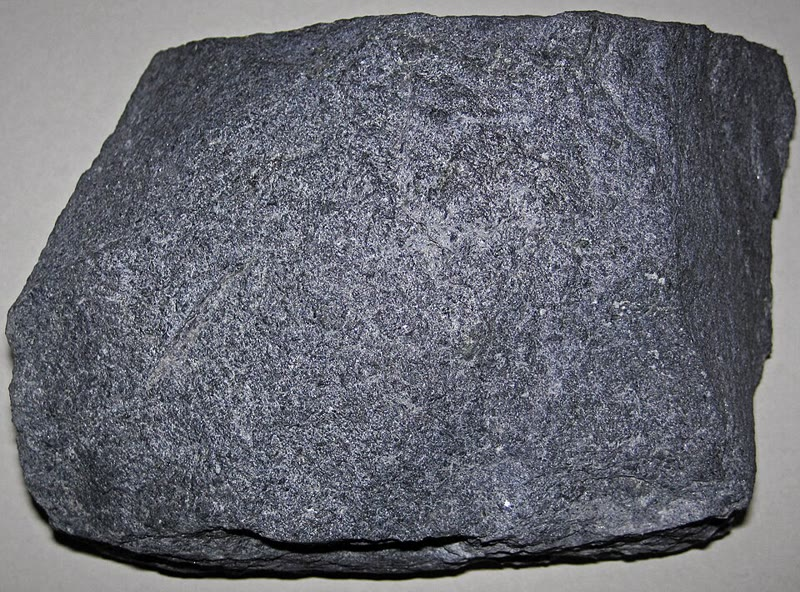
\includegraphics[height=4.4cm]{images/book2/g11-stjohn-blueschist.jpg}\hspace{0.03\linewidth}%
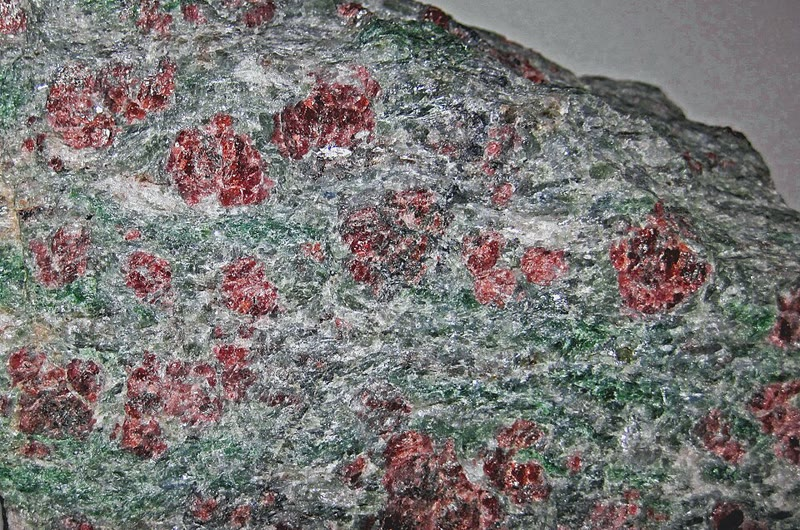
\includegraphics[height=4.4cm]{images/book2/g11-stjohn-eclogite.jpg}

{\small À esquerda: \omterm{def:g11:subduction-zones:eclogite}{xisto azul} da ilha de Santa Catalina, na Califórnia,
antiga \omterm{def:g11:ocean-ridges:oceanic-lithosphere}{crosta oceânica} enterrada numa \omterm{def:g11:subduction-zones:subduction}{zona de subducção}. À direita: \omterm{def:g11:subduction-zones:eclogite}{eclogito}
da Noruega, com granadas vermelhas em piroxênio verde. Fotografias James
St.~John (CC~BY~2.0).}
\end{omfigure}
% ledger: photo:g11-blueschist, photo:g11-eclogite

O \omterm{def:g11:subduction-zones:eclogite}{eclogito} é mais denso que o basalto; ele é até mais denso que o \omterm{def:g11:ocean-ridges:peridotite}{peridotito}
do manto, em cerca de \qty{6}{\percent}. Quando a sua crosta se transforma
em \omterm{def:g11:subduction-zones:eclogite}{eclogito}, a \omterm{def:g11:subduction-zones:slab}{laje} já não carrega uma camada leve por cima: a \omterm{def:g11:subduction-zones:slab}{laje} inteira
é mais densa que o manto em volta, e puxa com mais força. As rochas desse
tipo, trazidas de volta à superfície por movimentos posteriores, estão entre
as poucas testemunhas diretas do que acontece a dezenas de quilômetros de
profundidade numa \omterm{def:g11:subduction-zones:subduction}{zona de subducção}.
% ledger: hacker03:eclogite, photo:g11-eclogite

\begin{omfigure}
\begin{tikzpicture}[font=\footnotesize, scale=0.85]
  % subduction zone, a drawing, not to scale: slab top flat to x = -1, then bends to a 42-degree dip
  % coordinates computed once by a small script (scratch, not kept): slab top flat to x=-1, arc R=3 to a 42-degree dip
  \fill[omProp!10] (-7,-1.4) rectangle (7,-6.0);
  \fill[omSea!45] (-7,0) -- (-1,0) -- (1.6,0.8) -- (-7,0.8) -- cycle;
  \fill[lith peridotite] (-7.000,0.000) -- (-6.644,0.000) -- (-6.289,0.000) -- (-5.933,0.000) -- (-5.578,0.000) -- (-5.222,0.000) -- (-4.867,0.000) -- (-4.511,0.000) -- (-4.156,0.000) -- (-3.800,0.000) -- (-3.445,0.000) -- (-3.089,0.000) -- (-2.734,0.000) -- (-2.378,0.000) -- (-2.023,0.000) -- (-1.667,0.000) -- (-1.312,0.000) -- (-0.956,-0.000) -- (-0.602,-0.027) -- (-0.253,-0.094) -- (0.085,-0.203) -- (0.408,-0.351) -- (0.712,-0.536) -- (0.991,-0.756) -- (1.255,-0.994) -- (1.519,-1.232) -- (1.784,-1.470) -- (2.048,-1.707) -- (2.312,-1.945) -- (2.576,-2.183) -- (2.840,-2.421) -- (3.105,-2.659) -- (3.369,-2.897) -- (3.633,-3.135) -- (3.897,-3.373) -- (4.161,-3.611) -- (4.426,-3.848) -- (4.690,-4.086) -- (4.954,-4.324) -- (5.218,-4.562) -- (5.483,-4.800) -- (4.546,-5.840) -- (4.282,-5.603) -- (4.017,-5.365) -- (3.753,-5.127) -- (3.489,-4.889) -- (3.225,-4.651) -- (2.961,-4.413) -- (2.696,-4.175) -- (2.432,-3.937) -- (2.168,-3.699) -- (1.904,-3.461) -- (1.639,-3.224) -- (1.375,-2.986) -- (1.111,-2.748) -- (0.847,-2.510) -- (0.583,-2.272) -- (0.318,-2.034) -- (0.062,-1.803) -- (-0.087,-1.686) -- (-0.249,-1.587) -- (-0.421,-1.508) -- (-0.602,-1.450) -- (-0.788,-1.414) -- (-0.977,-1.400) -- (-1.312,-1.400) -- (-1.667,-1.400) -- (-2.023,-1.400) -- (-2.378,-1.400) -- (-2.734,-1.400) -- (-3.089,-1.400) -- (-3.445,-1.400) -- (-3.800,-1.400) -- (-4.156,-1.400) -- (-4.511,-1.400) -- (-4.867,-1.400) -- (-5.222,-1.400) -- (-5.578,-1.400) -- (-5.933,-1.400) -- (-6.289,-1.400) -- (-6.644,-1.400) -- (-7.000,-1.400) -- cycle;
  \fill[lith basalt] (-7.000,0.000) -- (-6.644,0.000) -- (-6.289,0.000) -- (-5.933,0.000) -- (-5.578,0.000) -- (-5.222,0.000) -- (-4.867,0.000) -- (-4.511,0.000) -- (-4.156,0.000) -- (-3.800,0.000) -- (-3.445,0.000) -- (-3.089,0.000) -- (-2.734,0.000) -- (-2.378,0.000) -- (-2.023,0.000) -- (-1.667,0.000) -- (-1.312,0.000) -- (-0.956,-0.000) -- (-0.602,-0.027) -- (-0.253,-0.094) -- (0.085,-0.203) -- (0.408,-0.351) -- (0.712,-0.536) -- (0.991,-0.756) -- (1.255,-0.994) -- (1.519,-1.232) -- (1.784,-1.470) -- (2.048,-1.707) -- (2.312,-1.945) -- (2.576,-2.183) -- (2.840,-2.421) -- (3.105,-2.659) -- (3.369,-2.897) -- (3.633,-3.135) -- (3.897,-3.373) -- (4.161,-3.611) -- (4.426,-3.848) -- (4.690,-4.086) -- (4.954,-4.324) -- (5.218,-4.562) -- (5.483,-4.800) -- (5.282,-5.023) -- (5.018,-4.785) -- (4.753,-4.547) -- (4.489,-4.309) -- (4.225,-4.071) -- (3.961,-3.833) -- (3.697,-3.596) -- (3.432,-3.358) -- (3.168,-3.120) -- (2.904,-2.882) -- (2.640,-2.644) -- (2.376,-2.406) -- (2.111,-2.168) -- (1.847,-1.930) -- (1.583,-1.692) -- (1.319,-1.455) -- (1.054,-1.217) -- (0.792,-0.980) -- (0.541,-0.783) -- (0.268,-0.616) -- (-0.023,-0.483) -- (-0.328,-0.385) -- (-0.642,-0.324) -- (-0.960,-0.300) -- (-1.312,-0.300) -- (-1.667,-0.300) -- (-2.023,-0.300) -- (-2.378,-0.300) -- (-2.734,-0.300) -- (-3.089,-0.300) -- (-3.445,-0.300) -- (-3.800,-0.300) -- (-4.156,-0.300) -- (-4.511,-0.300) -- (-4.867,-0.300) -- (-5.222,-0.300) -- (-5.578,-0.300) -- (-5.933,-0.300) -- (-6.289,-0.300) -- (-6.644,-0.300) -- (-7.000,-0.300) -- cycle;
  \fill[blue!30] (2.484,-2.100) -- (2.604,-2.208) -- (2.725,-2.317) -- (2.845,-2.425) -- (2.965,-2.533) -- (3.085,-2.642) -- (3.206,-2.750) -- (3.326,-2.858) -- (3.446,-2.967) -- (3.567,-3.075) -- (3.687,-3.183) -- (3.807,-3.292) -- (3.928,-3.400) -- (3.727,-3.623) -- (3.607,-3.515) -- (3.486,-3.406) -- (3.366,-3.298) -- (3.246,-3.190) -- (3.125,-3.081) -- (3.005,-2.973) -- (2.885,-2.865) -- (2.764,-2.756) -- (2.644,-2.648) -- (2.524,-2.540) -- (2.403,-2.431) -- (2.283,-2.323) -- cycle;
  \fill[lith eclogite] (3.928,-3.400) -- (4.057,-3.517) -- (4.187,-3.633) -- (4.316,-3.750) -- (4.446,-3.867) -- (4.576,-3.983) -- (4.705,-4.100) -- (4.835,-4.217) -- (4.964,-4.333) -- (5.094,-4.450) -- (5.223,-4.567) -- (5.353,-4.683) -- (5.483,-4.800) -- (5.282,-5.023) -- (5.152,-4.906) -- (5.023,-4.790) -- (4.893,-4.673) -- (4.764,-4.556) -- (4.634,-4.440) -- (4.504,-4.323) -- (4.375,-4.206) -- (4.245,-4.090) -- (4.116,-3.973) -- (3.986,-3.856) -- (3.857,-3.740) -- (3.727,-3.623) -- cycle;
  \draw[black!60] (-7.000,0.000) -- (-6.644,0.000) -- (-6.289,0.000) -- (-5.933,0.000) -- (-5.578,0.000) -- (-5.222,0.000) -- (-4.867,0.000) -- (-4.511,0.000) -- (-4.156,0.000) -- (-3.800,0.000) -- (-3.445,0.000) -- (-3.089,0.000) -- (-2.734,0.000) -- (-2.378,0.000) -- (-2.023,0.000) -- (-1.667,0.000) -- (-1.312,0.000) -- (-0.956,-0.000) -- (-0.602,-0.027) -- (-0.253,-0.094) -- (0.085,-0.203) -- (0.408,-0.351) -- (0.712,-0.536) -- (0.991,-0.756) -- (1.255,-0.994) -- (1.519,-1.232) -- (1.784,-1.470) -- (2.048,-1.707) -- (2.312,-1.945) -- (2.576,-2.183) -- (2.840,-2.421) -- (3.105,-2.659) -- (3.369,-2.897) -- (3.633,-3.135) -- (3.897,-3.373) -- (4.161,-3.611) -- (4.426,-3.848) -- (4.690,-4.086) -- (4.954,-4.324) -- (5.218,-4.562) -- (5.483,-4.800);
  \draw[black!60] (-7.000,-1.400) -- (-6.644,-1.400) -- (-6.289,-1.400) -- (-5.933,-1.400) -- (-5.578,-1.400) -- (-5.222,-1.400) -- (-4.867,-1.400) -- (-4.511,-1.400) -- (-4.156,-1.400) -- (-3.800,-1.400) -- (-3.445,-1.400) -- (-3.089,-1.400) -- (-2.734,-1.400) -- (-2.378,-1.400) -- (-2.023,-1.400) -- (-1.667,-1.400) -- (-1.312,-1.400) -- (-0.977,-1.400) -- (-0.788,-1.414) -- (-0.602,-1.450) -- (-0.421,-1.508) -- (-0.249,-1.587) -- (-0.087,-1.686) -- (0.062,-1.803) -- (0.318,-2.034) -- (0.583,-2.272) -- (0.847,-2.510) -- (1.111,-2.748) -- (1.375,-2.986) -- (1.639,-3.224) -- (1.904,-3.461) -- (2.168,-3.699) -- (2.432,-3.937) -- (2.696,-4.175) -- (2.961,-4.413) -- (3.225,-4.651) -- (3.489,-4.889) -- (3.753,-5.127) -- (4.017,-5.365) -- (4.282,-5.603) -- (4.546,-5.840);
  \draw[black!60] (5.483,-4.800) -- (4.546,-5.840);
  \fill[omLithGranite!55] (-1.000,0.000) -- (1.600,0.800) -- (7.000,0.800) -- (7.000,-1.600) -- (1.929,-1.600) -- (1.801,-1.485) -- (1.673,-1.370) -- (1.545,-1.255) -- (1.417,-1.140) -- (1.290,-1.025) -- (1.162,-0.910) -- (1.034,-0.795) -- (0.904,-0.682) -- (0.768,-0.577) -- (0.627,-0.479) -- (0.480,-0.390) -- (0.328,-0.310) -- (0.172,-0.238) -- (0.011,-0.176) -- (-0.152,-0.122) -- (-0.318,-0.078) -- (-0.487,-0.044) -- (-0.657,-0.020) -- (-0.828,-0.005) -- (-1.000,0.000) -- cycle;
  \fill[omLithAlluv] (-1.000,0.000) -- (0.550,0.470) -- (0.926,-0.700) -- (0.761,-0.571) -- (0.588,-0.455) -- (0.407,-0.350) -- (0.219,-0.259) -- (0.025,-0.180) -- (-0.174,-0.116) -- (-0.377,-0.065) -- (-0.583,-0.029) -- (-0.791,-0.007) -- (-1.000,0.000) -- cycle;
  \draw[black!60] (-1.000,0.000) -- (1.600,0.800) -- (7.000,0.800) -- (7.000,-1.600) -- (1.929,-1.600) -- (1.801,-1.485) -- (1.673,-1.370) -- (1.545,-1.255) -- (1.417,-1.140) -- (1.290,-1.025) -- (1.162,-0.910) -- (1.034,-0.795) -- (0.904,-0.682) -- (0.768,-0.577) -- (0.627,-0.479) -- (0.480,-0.390) -- (0.328,-0.310) -- (0.172,-0.238) -- (0.011,-0.176) -- (-0.152,-0.122) -- (-0.318,-0.078) -- (-0.487,-0.044) -- (-0.657,-0.020) -- (-0.828,-0.005) -- (-1.000,0.000);
  \draw[omThm!75, densely dashed, line width=0.7pt] (-7.000,-1.150) -- (-6.648,-1.150) -- (-6.296,-1.150) -- (-5.945,-1.150) -- (-5.593,-1.150) -- (-5.241,-1.150) -- (-4.889,-1.150) -- (-4.538,-1.150) -- (-4.186,-1.150) -- (-3.834,-1.150) -- (-3.482,-1.150) -- (-3.130,-1.150) -- (-2.779,-1.150) -- (-2.427,-1.150) -- (-2.075,-1.150) -- (-1.723,-1.150) -- (-1.372,-1.150) -- (-1.020,-1.150) -- (-0.796,-1.161) -- (-0.582,-1.198) -- (-0.374,-1.259) -- (-0.175,-1.344) -- (0.013,-1.452) -- (0.187,-1.581) -- (0.419,-1.788) -- (0.680,-2.023) -- (0.942,-2.259) -- (1.203,-2.494) -- (1.465,-2.730) -- (1.726,-2.965) -- (1.987,-3.200) -- (2.249,-3.436) -- (2.510,-3.671) -- (2.772,-3.907) -- (3.033,-4.142) -- (3.294,-4.377) -- (3.556,-4.613) -- (3.817,-4.848) -- (4.079,-5.083) -- (4.340,-5.319) -- (4.602,-5.554) -- (5.103,-4.997) -- (5.045,-4.944) -- (4.987,-4.892) -- (4.929,-4.839) -- (4.870,-4.787) -- (4.812,-4.734) -- (4.754,-4.682) -- (4.695,-4.629) -- (4.637,-4.577) -- (4.579,-4.524) -- (4.520,-4.472) -- (4.462,-4.419) -- (4.404,-4.367) -- (4.346,-4.315) -- (4.287,-4.262) -- (4.229,-4.210) -- (4.171,-4.157) -- (4.112,-4.105) -- (4.054,-4.052) -- (3.996,-4.000) -- (3.937,-3.947) -- (3.879,-3.895) -- (3.821,-3.842) -- (3.763,-3.790) -- (3.704,-3.737) -- (3.646,-3.685) -- (3.588,-3.632) -- (3.529,-3.580) -- (3.471,-3.527) -- (3.413,-3.475) -- (3.355,-3.422) -- (3.296,-3.370) -- (3.238,-3.317) -- (3.180,-3.265) -- (3.121,-3.212) -- (3.063,-3.160) -- (3.005,-3.107) -- (2.946,-3.055) -- (2.888,-3.002) -- (2.830,-2.950) -- (2.772,-2.897) -- (7.000,-2.897);
  \foreach \p in {(-0.72,-0.22),(-0.46,-0.36),(-0.18,-0.37),(0.05,-0.55),(0.29,-0.67),(0.63,-0.66),(0.87,-0.82),(0.91,-1.23),(1.27,-1.29),(1.50,-1.49),(1.55,-1.89),(1.90,-1.96),(2.04,-2.25),(2.35,-2.36),(2.54,-2.61),(2.88,-2.69),(2.99,-3.02),(3.16,-3.28),(3.47,-3.40),(3.65,-3.66),(3.89,-3.84),(4.26,-3.89),(4.32,-4.27),(4.59,-4.43),(4.88,-4.56),(5.17,-4.70)} \fill[black] \p circle (1.3pt);
  % volcanic arc above the slab, back-arc stretched
  \fill[black!70] (3.35,0.8) -- (3.7,1.4) -- (4.05,0.8) -- cycle;
  \draw[black!45, dashed] (5.2,0.8) -- (5.2,-1.6); \draw[black!45, dashed] (6.6,0.8) -- (6.6,-1.6);
  \draw[{Stealth[length=4pt]}-{Stealth[length=4pt]}, black!70] (5.35,-0.7) -- (6.45,-0.7);
  % motion arrows
  \draw[-{Stealth[length=5pt]}, line width=1pt] (-5.6,0.4) -- (-3.6,0.4);
  \draw[-{Stealth[length=5pt]}, line width=1pt] (1.77,-4.01) -- (2.88,-5.01);
  % labels
  \draw[black!60] (-1.0,0.02) -- (-1.8,1.05);
  \node[anchor=south] at (-1.8,1.05) {fossa};
  \draw[black!60] (0.1,0.12) -- (0.5,1.05);
  \node[anchor=south, align=center] at (0.6,1.05) {sedimentos\\raspados};
  \node[anchor=south] at (2.35,0.85) {antearco};
  \node[anchor=south] at (3.7,1.4) {arco vulcânico};
  \node[anchor=south] at (5.9,0.85) {retroarco};
  \node[anchor=south] at (-5.4,0.82) {fundo oceânico que vai para a fossa};
  \draw[black!60] (-7.0,-0.15) -- (-7.25,-0.15);
  \node[anchor=east] at (-7.25,-0.15) {crosta oceânica};
  \draw[black!60] (-7.0,-0.85) -- (-7.25,-0.85);
  \node[anchor=east, align=right] at (-7.25,-0.85) {parte mantélica\\da litosfera};
  \node at (-3.5,-3.6) {astenosfera};
  \node[rotate=-42] at (3.98,-4.46) {laje};
  \draw[black!60] (3.35,-2.65) -- (4.3,-2.35);
  \node[anchor=west] at (4.3,-2.35) {xisto azul};
  \draw[black!60] (5.1,-4.3) -- (5.75,-4.6);
  \node[anchor=west] at (5.75,-4.6) {eclogito};
  \node[anchor=north east, text=omThm!80!black, align=right] at (7,-2.95) {linha de mesma\\temperatura};
  \fill[black] (-6.8,-5.55) circle (1.3pt);
  \node[anchor=west] at (-6.65,-5.55) {terremotos};
\end{tikzpicture}

{\small Uma \omterm{def:g11:subduction-zones:subduction}{zona de subducção} (um desenho, fora de escala). A \omterm{def:g11:ocean-ridges:oceanic-lithosphere}{litosfera
oceânica} antiga se dobra para baixo na fossa e afunda sob a placa que se
sobrepõe. Os sedimentos raspados da sua superfície se empilham contra a
borda da placa que se sobrepõe; os terremotos seguem a \omterm{def:g11:subduction-zones:slab}{laje} que afunda; a sua
crosta se transforma em \omterm{def:g11:subduction-zones:eclogite}{xisto azul}, e depois em \omterm{def:g11:subduction-zones:eclogite}{eclogito}. A \omterm{def:g11:subduction-zones:slab}{laje} continua
mais fria que o manto em volta: as linhas de mesma temperatura são
arrastadas para baixo ao longo dela. Uma linha de vulcões, o arco vulcânico,
fica acima da \omterm{def:g11:subduction-zones:slab}{laje}.}
\end{omfigure}
% volcanic arc above the slab: told only, defined and sourced in g12.04

\section{A anatomia de uma zona de subducção}

Do oceano ao continente, ou ao oceano seguinte, uma \omterm{def:g11:subduction-zones:subduction}{zona de subducção} tem
sempre as mesmas partes.

\begin{itemize}
  \item A \emph{fossa}, onde a placa que afunda se dobra para baixo: os
        lugares mais profundos dos oceanos.
  \item O \emph{antearco}, entre a fossa e a linha de vulcões. A sua borda é
        uma pilha de sedimentos raspados da placa que afunda; abaixo dele, as
        duas placas deslizam uma contra a outra ao longo do limite de placas,
        uma falha de mergulho suave na qual acontecem grandes terremotos,
        como o de 2011 ao largo do Japão (exemplo abaixo).
  \item O \emph{arco vulcânico}, uma linha de vulcões paralela à fossa, em
        ilhas (Tonga, as Marianas, o Japão) ou num continente (os Andes); por
        que ele se forma é o assunto do \cref{ch:g12:subduction-magmatism}.
  \item Atrás de alguns arcos, um \emph{retroarco}, onde a placa que se
        sobrepõe é estirada; atrás de Tonga, ele está sendo aberto.
\end{itemize}
% ledger: bevis95:tonga (back-arc extension at Tonga); usgs:tohoku (largest earthquakes on the
% plate boundary: example below)

Atrás de Tonga, o estiramento do retroarco leva o próprio arco em direção à
placa do Pacífico, como mostrou o posicionamento por satélite. A taxa com que os dois lados da fossa de Tonga convergem
é portanto maior que a velocidade de qualquer uma das placas: pelo modelo
PB2002, cerca de \qty{17}{cm} por ano perto de \ang{20}~Sul.
% values: tonga_rate 168.0 (mean of the PB2002 TO/PA steps within 100 km of the profile);
% PB2002 steps along Tonga: 104 to 237 mm/yr; ledger data:pb2002, bevis95:tonga

\begin{example}[O terremoto de Tōhoku, 2011]\label{ex:g11:subduction-zones:tohoku}
Em 11~de março de 2011, um terremoto de magnitude 9.1 atingiu o largo da
costa nordeste de Honshu, no Japão. Ele aconteceu a cerca de \qty{25}{km} de
profundidade, no próprio limite de placas, onde a placa do Pacífico, que se
move para oeste a cerca de \qty{83}{mm} por ano em relação à placa que
carrega o norte do Japão, afunda sob ela na fossa do Japão. Os dois lados da
falha deslizaram um em relação ao outro até 50 a \qty{60}{m}, numa área de
cerca de \qty{400}{km} de comprimento e \qty{150}{km} de largura. O fundo do
mar acima se moveu junto, e provocou um tsunami que subiu até \qty{38}{m} de
altura na costa; pelo menos \num{15703} pessoas morreram e \num{4647} ficaram
desaparecidas. A mesma costa tinha sido atingida por tsunamis desta \omterm{def:g11:subduction-zones:subduction}{zona de
subducção} em 1611, 1896 e 1933, e talvez por um tão grande quanto o de 2011
no ano de 869.
\end{example}
% ledger: usgs:tohoku

\begin{omfigure}
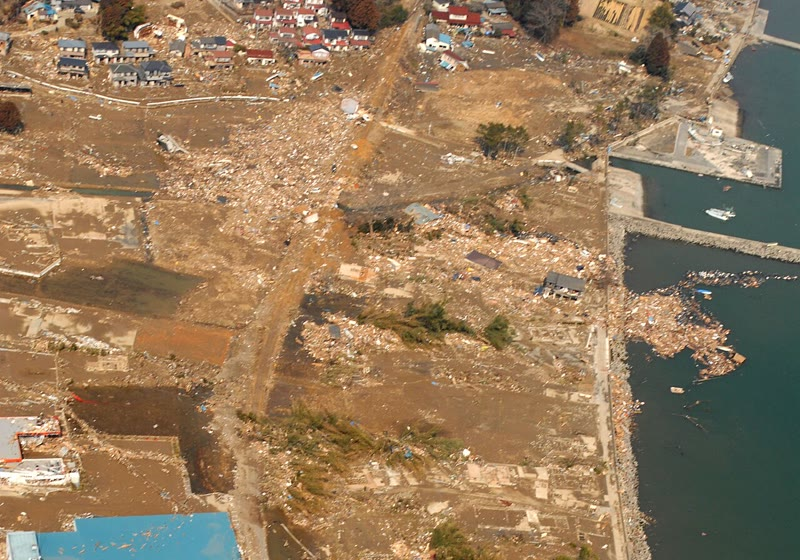
\includegraphics[width=0.78\linewidth]{images/book2/g11-usn-tsunami-kesennuma.jpg}

{\small O porto pesqueiro de Kesennuma, na costa nordeste do Japão, dois dias
depois do tsunami de 11~de março de 2011. Fotografia Dylan McCord, U.S. Navy
(domínio público).}
\end{omfigure}
% ledger: photo:g11-tsunami

\section{Exercícios}

\begin{exercise}[$\star$]\label{exo:g11:subduction-zones:1}
Defina a \omterm{def:g11:subduction-zones:subduction}{subducção} e uma \omterm{def:g11:subduction-zones:subduction}{zona de subducção}. Que tipo de \omterm{def:g11:lithosphere-asthenosphere:lithosphere}{litosfera} afunda
numa \omterm{def:g11:subduction-zones:subduction}{zona de subducção}, e por que esse tipo?
\end{exercise}

\begin{exercise}[$\star$]\label{exo:g11:subduction-zones:2}
Usando o mapa-múndi dos terremotos por profundidade: (1) cite três regiões
com terremotos de mais de \qty{300}{km} de profundidade; (2) de que lado de
uma fossa ficam os terremotos profundos? (3) Ao longo da Dorsal
Mesoatlântica, a que profundidade ficam os terremotos?
\end{exercise}

\begin{exercise}[$\star$]\label{exo:g11:subduction-zones:3}
O catálogo contém \num{7031} terremotos de magnitude 6 ou mais, dos quais
\qty{21}{\percent} têm mais de \qty{70}{km} de profundidade e
\qty{6.9}{\percent} mais de \qty{300}{km}. Quantos terremotos isso dá em cada
caso?
\end{exercise}

\begin{exercise}[$\star$]\label{exo:g11:subduction-zones:4}
Defina o \omterm{def:g11:subduction-zones:eclogite}{xisto azul} e o \omterm{def:g11:subduction-zones:eclogite}{eclogito}. O que os dois têm em comum com o basalto
da \omterm{def:g11:ocean-ridges:oceanic-lithosphere}{crosta oceânica}? O que difere?
\end{exercise}

\begin{exercise}[$\star$]\label{exo:g11:subduction-zones:5}
Liste as partes de uma \omterm{def:g11:subduction-zones:subduction}{zona de subducção} em ordem, do fundo oceânico que se
move em direção à fossa até o retroarco, dizendo numa linha o que acontece
em cada uma.
\end{exercise}

\begin{exercise}[$\star\star$]\label{exo:g11:subduction-zones:6}
No corte dos Andes, a reta que acompanha os terremotos passa a
\qty{135}{km} de profundidade a \qty{300}{km} da fossa e a \qty{508}{km} de
profundidade a \qty{800}{km}. Calcule o mergulho da \omterm{def:g11:subduction-zones:slab}{laje}.
\end{exercise}

\begin{exercise}[$\star\star$]\label{exo:g11:subduction-zones:7}
Uma \omterm{def:g11:subduction-zones:slab}{laje} reta começa numa fossa e mergulha a \ang{45}. (1) A que
profundidade ela está a \qty{300}{km} da fossa? (2) A que distância da fossa
ela chega a \qty{670}{km}? (3) Que comprimento de \omterm{def:g11:subduction-zones:slab}{laje} fica entre a fossa e
\qty{670}{km}?
\end{exercise}

\begin{exercise}[$\star\star$]\label{exo:g11:subduction-zones:8}
As velocidades médias das placas são, em milímetros por ano: Cocos 74.6,
Nazca 70.0, Pacífico 65.5, Austrália 63.1, Mar das Filipinas 52.6 (com
\omterm{def:g11:subduction-zones:slab}{lajes}); Arábia 47.6, Somália 31.0, Núbia 29.2, Eurásia 22.8, América do Norte
19.8, Antártida 15.2, Caribe 14.9, América do Sul 10.6 (sem). (1) Calcule a
média de cada grupo e a razão entre elas. (2) O que isso sugere sobre a
força que move as placas?
\end{exercise}

\begin{exercise}[$\star\star$]\label{exo:g11:subduction-zones:9}
Em 2011, a falha ao largo do Japão deslizou até 50 a \qty{60}{m}. A placa do
Pacífico se aproxima a \qty{83}{mm} por ano. (1) A quantos anos de movimento
da placa corresponde um deslizamento de \qty{50}{m}, e depois de
\qty{60}{m}? (2) Compare com o tempo desde 869, um possível terremoto
anterior do mesmo tamanho.
\end{exercise}

\begin{exercise}[$\star\star$]\label{exo:g11:subduction-zones:10}
O fundo oceânico que chega à fossa do Japão tem cerca de 133 milhões de
anos, o que chega a Tonga cerca de 99 e o que chega aos Andes cerca de 49.
(1) Usando as leis do \cref{ch:g11:ocean-ridges} ($2500 + 350\sqrt{t}$ para
$t \le 70$, $6400 - 3200\,e^{-t/62.8}$ além disso), encontre a profundidade de
cada um. (2) Qual é a \omterm{def:g11:lithosphere-asthenosphere:lithosphere}{litosfera} mais fria e mais densa?
\end{exercise}

\begin{exercise}[$\star\star$]\label{exo:g11:subduction-zones:11}
O basalto da \omterm{def:g11:ocean-ridges:oceanic-lithosphere}{crosta oceânica} tem uma densidade de cerca de
\qty{2900}{kg/m^3}, o manto em volta da \omterm{def:g11:subduction-zones:slab}{laje} \qty{3380}{kg/m^3}, e o
\omterm{def:g11:subduction-zones:eclogite}{eclogito} é \qty{6}{\percent} mais denso que o manto. (1) Encontre a
densidade do \omterm{def:g11:subduction-zones:eclogite}{eclogito}. (2) Em que porcentagem a densidade da crosta aumenta
quando ela se transforma em \omterm{def:g11:subduction-zones:eclogite}{eclogito}? (3) Antes e depois, a crosta é mais
leve ou mais densa que o manto, e em quanto?
\end{exercise}

\begin{exercise}[$\star\star\star$]\label{exo:g11:subduction-zones:12}
O calor se espalha por condução por uma distância de cerca de
$\sqrt{\kappa t}$ num tempo $t$, com $\kappa = \qty{1e-6}{m^2/s}$ para a
rocha. (1) Calcule essa distância para 6 milhões de anos ($1~\text{ano} \approx \qty{3.16e7}{s}$). (2) Compare-a
com a espessura de uma \omterm{def:g11:subduction-zones:slab}{laje}, cerca de \qty{100}{km}. (3) Explique por que
podem acontecer terremotos dentro de uma \omterm{def:g11:subduction-zones:slab}{laje} a \qty{600}{km} enquanto o
manto em volta escoa.
\end{exercise}
% ledger: england:kelvin (kappa 1e-6 m2/s)

\begin{exercise}[$\star\star\star$]\label{exo:g11:subduction-zones:13}
Sob os Andes a \ang{21}~Sul, a reta do corte chega a \qty{670}{km} a
\qty{1017}{km} da fossa, e as placas convergem a \qty{64}{mm} por ano.
(1) Estime o comprimento da \omterm{def:g11:subduction-zones:slab}{laje} da fossa até \qty{670}{km}. (2) Quanto
tempo um pedaço de fundo oceânico leva para chegar a \qty{670}{km}?
(3) Compare com Tonga, onde a mesma viagem leva cerca de 6 milhões de anos.
\end{exercise}

\begin{exercise}[$\star\star\star$]\label{exo:g11:subduction-zones:14}
Tome uma \omterm{def:g11:subduction-zones:slab}{laje} de \qty{100}{km} de espessura, mais densa que o manto em volta
em \qty{36}{kg/m^3} em média, e de \qty{1000}{km} de comprimento, sob uma
fossa. (1) Calcule o excesso de massa da \omterm{def:g11:subduction-zones:slab}{laje} para cada metro de fossa.
(2) Calcule o seu peso, com $g = \qty{9.8}{m/s^2}$. (3) Por que essa força
pode puxar a placa inteira?
\end{exercise}

\begin{exercise}[$\star\star\star$]\label{exo:g11:subduction-zones:15}
Ao longo da fossa de Tonga, o modelo PB2002 dá uma convergência de
\qty{104}{mm} por ano a \ang{23.6}~Sul e de \qty{237}{mm} por ano a
\ang{16.5}~Sul. (1) A que distância estão os dois pontos, ao longo de um
meridiano ($\ang{1} \approx \qty{111}{km}$)? (2) Quanto a taxa cresce a cada
cem quilômetros? (3) A placa do Pacífico se move a mais ou menos a mesma
velocidade nos dois pontos. O que o outro lado da fossa, o arco de Tonga,
deve estar fazendo?
\end{exercise}

\section{Problema: a laje de Tonga}

\begin{problem}[{Problema de fim de semana --- da fossa a \qty{670}{km}}]
\label{pb:g11:subduction-zones:1}
% values: tonga fit -23.568 + 0.91068 x; tonga_rate 168.0 mm/yr; tonga_age 98.8;
% x670 761.6; path 1014; time 6.04 Myr; tonga_maxdepth 670.8 (slab_sections.py);
% MKEA 69 mm/yr (plate_velocities.py); kappa england:kelvin; eclogite hacker03:eclogite
Sob a fossa de Tonga, a placa do Pacífico afunda para oeste. Use o corte de
Tonga deste capítulo, cuja reta é $z = -24 + 0.91\,x$ (os dois em
quilômetros, com $x$ medido da fossa em direção ao arco).

\medskip
\noindent\textbf{Parte I --- O corte de terremotos.}
\begin{enumerate}
  \item Qual é a profundidade do terremoto mais profundo do corte?
  \item Por que não há terremotos profundos do lado oceânico da fossa?
  \item Calcule a profundidade da reta em $x = 300$ e $x = 700$, e depois o
        mergulho da \omterm{def:g11:subduction-zones:slab}{laje}.
  \item A que distância horizontal da fossa a \omterm{def:g11:subduction-zones:slab}{laje} está a \qty{100}{km} de
        profundidade? E a \qty{400}{km}?
  \item A reta passa \qty{24}{km} acima da fossa em $x = 0$. O que isso diz
        sobre a forma da \omterm{def:g11:subduction-zones:slab}{laje} perto da fossa?
\end{enumerate}

\medskip
\noindent\textbf{Parte II --- A convergência.}
\begin{enumerate}[resume]
  \item As placas convergem através da fossa a cerca de \qty{168}{mm} por
        ano. Converta em centímetros por ano e em quilômetros por milhão de
        anos.
  \item A placa do Pacífico se move sobre o Havaí a cerca de \qty{69}{mm}
        por ano. Quantas vezes mais rápida é a convergência em Tonga?
  \item Usando a soma das velocidades relativas, explique como a
        convergência pode superar a velocidade da placa do Pacífico.
  \item O fundo que chega à fossa tem cerca de 99 milhões de anos. A que
        profundidade ele fica (lei exponencial do \cref{ch:g11:ocean-ridges})?
  \item Por que uma \omterm{def:g11:lithosphere-asthenosphere:lithosphere}{litosfera} assim pode afundar sozinha?
\end{enumerate}

\medskip
\noindent\textbf{Parte III --- Descer até \qty{670}{km}.}
\begin{enumerate}[resume]
  \item A que distância horizontal da fossa a reta chega a \qty{670}{km}?
  \item Estime o comprimento da \omterm{def:g11:subduction-zones:slab}{laje} da fossa até esse ponto, tratando-a
        como reta.
  \item Quanto tempo um pedaço de fundo oceânico leva para percorrer esse
        comprimento a \qty{168}{mm} por ano?
  \item Quanto tempo levaria aos \qty{69}{mm} por ano da placa do Pacífico
        sobre o Havaí?
  \item No caminho, a crosta da \omterm{def:g11:subduction-zones:slab}{laje} se transforma em \omterm{def:g11:subduction-zones:eclogite}{eclogito},
        \qty{6}{\percent} mais denso que o manto a \qty{3380}{kg/m^3}. Qual
        é a sua densidade, e o que isso muda para a \omterm{def:g11:subduction-zones:slab}{laje}?
\end{enumerate}

\medskip
\noindent\textbf{Parte IV --- Uma laje fria num manto quente.}
\begin{enumerate}[resume]
  \item Durante o tempo da questão~13, o calor se espalha por condução por
        cerca de $\sqrt{\kappa t}$, com $\kappa = \qty{1e-6}{m^2/s}$. Calcule
        essa distância.
  \item Compare-a com a espessura da \omterm{def:g11:subduction-zones:slab}{laje}, cerca de \qty{100}{km}. A \omterm{def:g11:subduction-zones:slab}{laje}
        ainda está fria por dentro quando chega a \qty{670}{km}?
  \item Por que isso explica os terremotos a \qty{600}{km} e mais sob
        Tonga?
  \item Que mudança no manto as ondas sísmicas revelaram perto de
        \qty{670}{km} (\cref{ch:g11:seismic-structure})?
  \item Conclua: quanto tempo o fundo oceânico do Pacífico leva para ir da
        fossa de Tonga até \qty{670}{km} de profundidade?
\end{enumerate}
\end{problem}
